	\documentclass[aspectratio=43]{beamer}
\usepackage[latin1]{inputenc}
\usepackage{amsmath}
\usepackage{amsfonts}
\usepackage{amssymb}
\usepackage{makeidx}
\usepackage{graphicx}
\usepackage{array}

% Customization
\mode<presentation>{
	\usetheme{CambridgeUS}
	\usecolortheme{dolphin}
	\setbeamertemplate{navigation symbols}{}
}

% Define colors
\definecolor{darkgreen}{rgb}{0.0, 0.5, 0.13}
\definecolor{darkblue}{rgb}{0.0, 0.0, 0.55}
\definecolor{darkred}{rgb}{0.55, 0.0, 0.0}

% Title and author
\title[Higgs boson production at the LHC]{Higgs boson production at the LHC}
\author{\textbf {Jes\'us Urtasun Elizari}}
%\institute{\textbf {University of Milan}}
\date{Milan, February 2022}

\begin{document}

% Front slide
\begin{frame}

	%\maketitle
	\vspace{1.0 cm}
	
	\center{\color{blue}Higgs boson production at the Large Hadron Collider:\\
		accurate theoretical predictions at higher orders in QCD}
	
	\vspace{0.25 cm}
	\center{Jes\'us Urtasun Elizari}
	\center{PhD presentation - Milan, February 25th, 2022}

	\begin{figure}
		\minipage{1\textwidth}
		
\includegraphics[width = 3.0 cm]{plots/front_page/unimi.png}
		\hfill
		
\includegraphics[width = 3.0 cm]{plots/front_page/n3pdf.png}
		\hfill
		
\includegraphics[width = 3.0 cm]{plots/front_page/erc.png}
		\endminipage
	\end{figure}

	\vspace{1.0 cm}
	
	{\scriptsize \color{blue} This project has received funding from the European Union$'$s Horizon 2020 research and innovation program under grant agreement No 740006.}

\end{frame}

% Introduction
\begin{frame}

	\frametitle{Outline}
	
	\begin{enumerate}
		\item {\color{blue}Introduction to QCD}
		\begin{itemize}
			\item A historical approach
			\item Asymptotic freedom and pQCD
		\end{itemize}
		\item {\color{blue}QCD and collider physics}
		\begin{itemize}
			\item QCD Factorization
			\item Partonic cross section and perturbative QCD
		\end{itemize}
		\item {\color{blue}All order perturbative resummation}
		\begin{itemize}
			\item Higher order radiative corrections
			\item Resummation of large logarithmic corrections
			\item Resummed, asymptotic and fixed-order
		\end{itemize}
		\item {\color{blue}Precise and fast predictions for Higgs boson physics}
		\begin{itemize}
			\item Higgs production at the LHC
			\item HTurbo numerical code
			\item Preliminary results $\&$ Conclusions
		\end{itemize}
	\end{enumerate}
	
\end{frame}

%
% Introduction ...........................................................................
%

%
% Part 1 .................................................................................
% QCD and collider pysics ................................................................
%

% QCD and collider physics
\begin{frame}

	\center{\color{blue}Part I \\ QCD and collider physics}

\end{frame}

% QCD and the strong interactions
\begin{frame}

	\frametitle{Introduction}
	\framesubtitle{QCD and the strong interactions}
	
	\begin{itemize}
		\item \footnotesize The parton model
		\item \footnotesize QCD is the theory of the strong interactions
		\item \footnotesize Predictions in QFTs are done by computing cross sections
		\item \footnotesize Experiments for high energy physics are done at the LHC
	\end{itemize}

\end{frame}

% QCD and the strong interactions
\begin{frame}

	\frametitle{Introduction}
	\framesubtitle{QCD and the strong interactions}
	
	How to explore proton's inner structure?

	\begin{figure}
		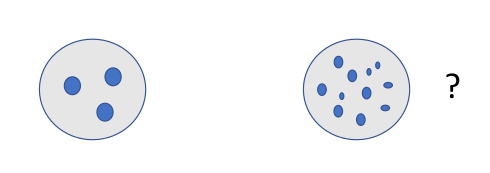
\includegraphics[width = 0.5\linewidth]{plots/part1/intro/protons.png}
	\end{figure}
	
	
	\begin{itemize}
		\item \footnotesize Point-like projectile on the object $\longrightarrow$ DIS
		\item \footnotesize Smash the two objects $\longrightarrow$ LHC physics
	\end{itemize}
	
	{\color{blue} \footnotesize "A way to analyze high energy collisions is to consider any hadron as a composition of point-like constituents $\longrightarrow$ \textbf{partons"} } R.Feynman, 1969 

\end{frame}

% Asymptotic freedom and pQCD
\begin{frame}

	\frametitle{QCD and collider physics}
	\framesubtitle{Asymptotic freedom and pQCD}

	\begin{columns}	
		
		\column{0.3\textwidth}
		
		\begin{figure}

			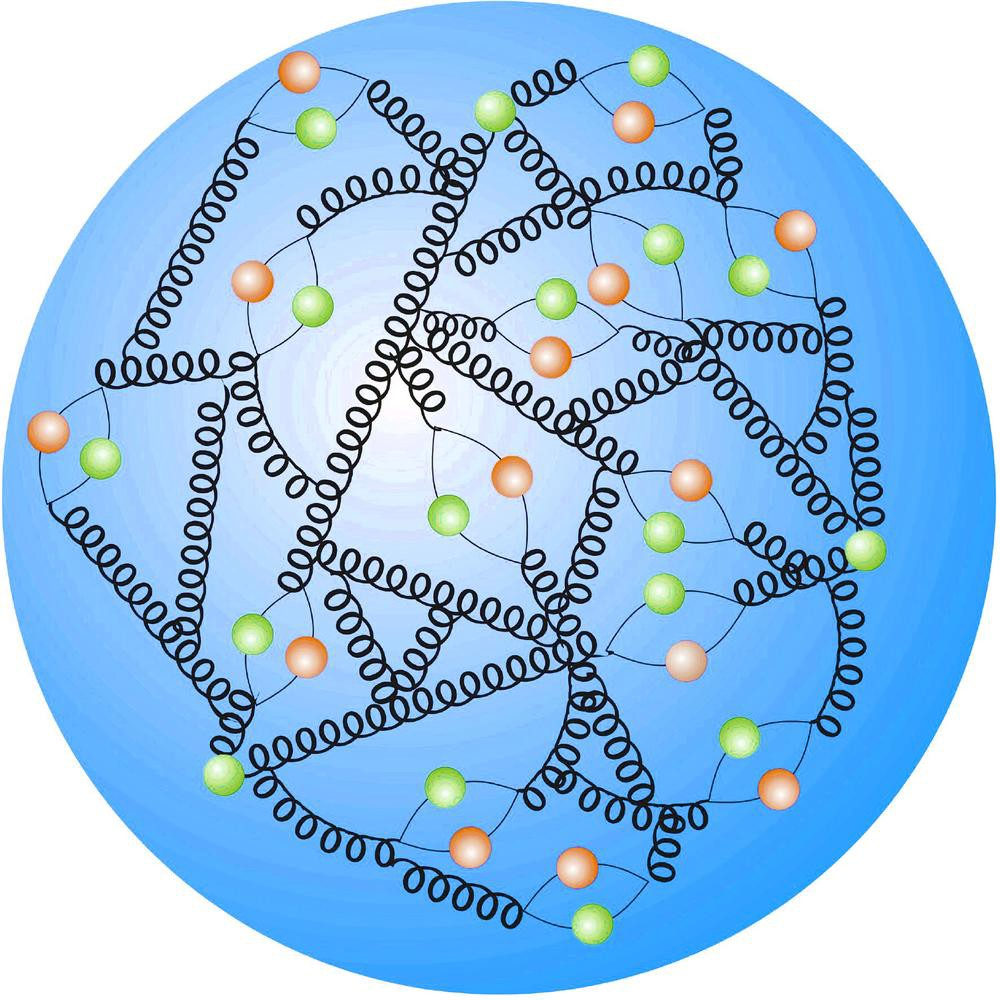
\includegraphics[width = 2 cm]{plots/part1/intro/proton2.jpg}
		\end{figure}
		
		\column{0.7\textwidth}
		
		\begin{itemize}
			\item \footnotesize QCD and QFTs, coupling strength changes with energy
			\item \footnotesize Charge a particle feels depends on the scale
			\item \footnotesize QED
		\end{itemize}
		
	\end{columns}
	
	\vspace{1cm}
	\center \footnotesize QCD is strongly coupled at short scales $\longrightarrow$ confinement
	\center \footnotesize \color{red} Non-perturbative physics

\end{frame}

%Asymptotic freedom and pQCD
\begin{frame}
	
	\frametitle{QCD and collider physics}
	\framesubtitle{Asymptotic freedom and pQCD}
	
	\begin{itemize}
		\item \footnotesize Running coupling given by Renormalization Group Equation (RGE)
		\begin{equation}
		{\color{blue}\mu\frac{d\alpha_{s}(\mu)}{d\mu} = \beta(\alpha_{s}(\mu)) = -\sum_{n = 0}^{\infty} \beta_{n} \Big( \frac{\alpha_{s}}{\pi} \Big)^{n + 1}} \nonumber
		\end{equation}
		\item \footnotesize Coupling {\color{blue}$\alpha_{s}$} evolves with scale {\color{blue}$\mu$} as given by RGE $\rightarrow$ LO behavior driven by $\beta_{0}$
		\item \footnotesize $\beta_{0}^{\textrm{QED}} < 0 \implies$ strongly coupled at large energies, {\color{blue}UV divergent}
		\item $\beta_{0}^{\textrm{QCD}} > 0 \implies$ weakly coupled at large energies, {\color{red}IR divergent}
	\end{itemize}

\end{frame}

% Asymptotic freedom and pQCD
\begin{frame}

	\frametitle{QCD and collider physics}
	\framesubtitle{Asymptotic freedom and pQCD}
	
	\begin{columns}	
		
		\column{0.5\textwidth}
		
		\begin{figure}
			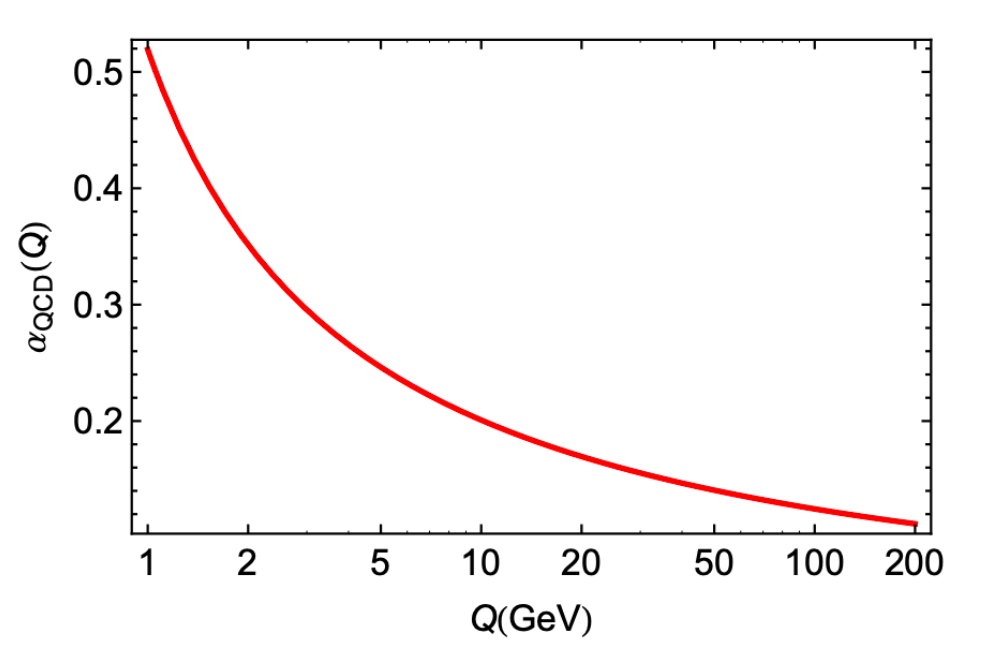
\includegraphics[width = 5 cm]{plots/part1/chapter1/qcd_running_coupling.png}
		\end{figure}
		
		\column{0.5\textwidth}
		
		\begin{itemize}
			\item \footnotesize Running coupling given by Renormalization Group Equation (RGE)
			\begin{equation}
			\alpha_{s}(\mu) = \frac{1}{\beta_{0} \log\big( \frac{\mu^{2}}{\Lambda_{\textrm{QCD}}^{2}}\big)} \nonumber
			\end{equation}
			\item \footnotesize $\beta_{0}$ LO of the $\beta$ function, is $ > 0$
			\item \footnotesize $\Lambda_{\textrm{QCD}}$, parameter that defines value of the coupling at large scales
		\end{itemize}
		
	\end{columns}
	
	\vspace{1cm}
	\center \footnotesize QCD is weakly coupled for $\mu >> \Lambda_{\textrm{QCD}} \longrightarrow$ asymptotically free
	\center \footnotesize \color{red} Perturbative Quantum Chromodynamics (pQCD)

\end{frame}

% Hadronic processes and factorization
\begin{frame}

	\frametitle{QCD and collider physics}
	\framesubtitle{Hadronic processes and factorization}
	
	\vspace{0.4 cm}
	
	\begin{figure}
		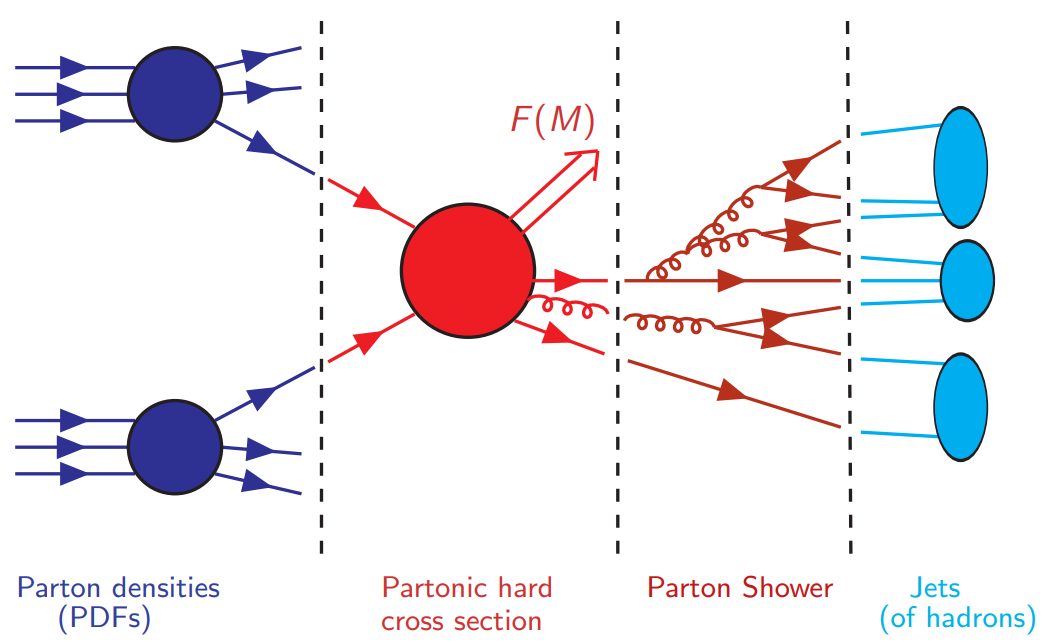
\includegraphics[width = 7 cm]{plots/part1/chapter2/factorization_1.png}
	\end{figure}
	
	\footnotesize Compute hadronic cross sections is a {\color{red}hard problem} $\longrightarrow$ {\color{blue} QCD Factorization}
	
	\begin{equation}
		\sigma^{\textrm{F}}(p_{1}, p_{2}) =
		\int_{0}^{1} dx_{1} dx_{2} \; {\color{blue} f_{\alpha}(x_{1}, \mu_{F}^{2}) \ast f_{\beta}(x_{2}, \mu_{F}^{2})}
		\; \ast \;  
		{\color{red}\hat{\sigma}^{\textrm{F}}_{\alpha \beta}(x_{1}p_{1}, x_{2}p_{2}, \alpha_{s}(\mu_{R}^{2}), \mu_{F}^{2})} \nonumber
	\end{equation}

\end{frame}

% Hadronic processes and factorization
\begin{frame}

	\frametitle{QCD and collider physics}
	\framesubtitle{Hadronic processes and factorization}
	
	\begin{figure}
		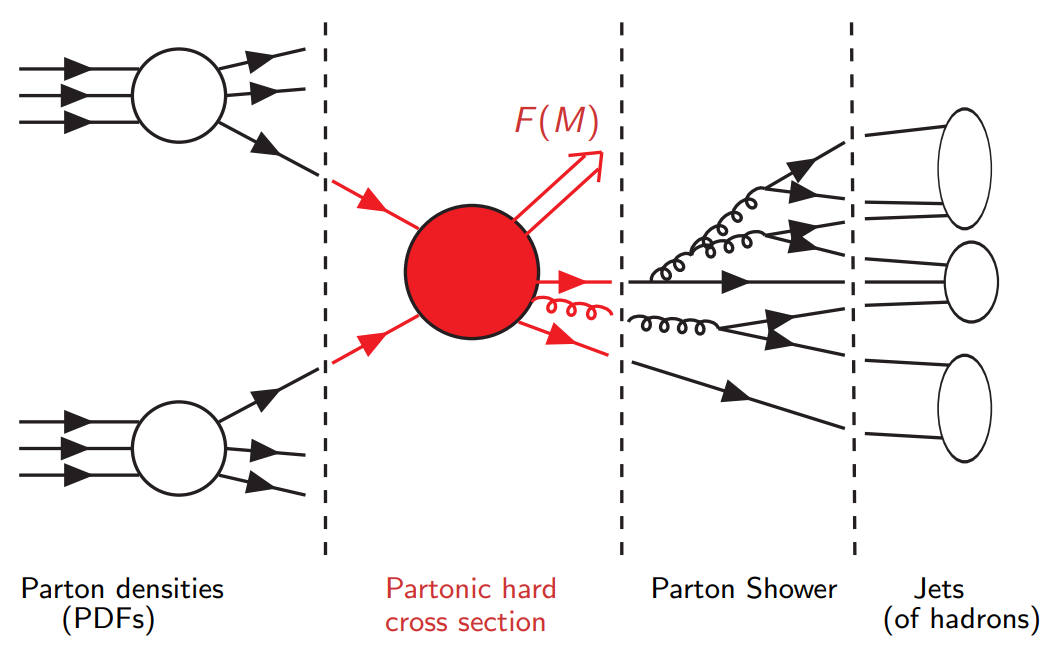
\includegraphics[width = 7 cm]{plots/part1/chapter2/factorization_2.png}
	\end{figure}
	
	\begin{itemize}
		\item \footnotesize Parton densities (PDFs) ${\color{blue} f_{\alpha}(x_{i}, \mu_{F}^{2})}$: non perturbative but universal
		\item \footnotesize Partonic cross section {\color{red}$\hat{\sigma}^{\textrm{F}}_{\alpha \beta}$}: process dependent but computable as perturbative series in $\alpha_{s}$
	\end{itemize}

\end{frame}

% Parton densities
\begin{frame}
	
	\frametitle{QCD and collider physics}
	\framesubtitle{Parton densities}
	
	\begin{figure}
		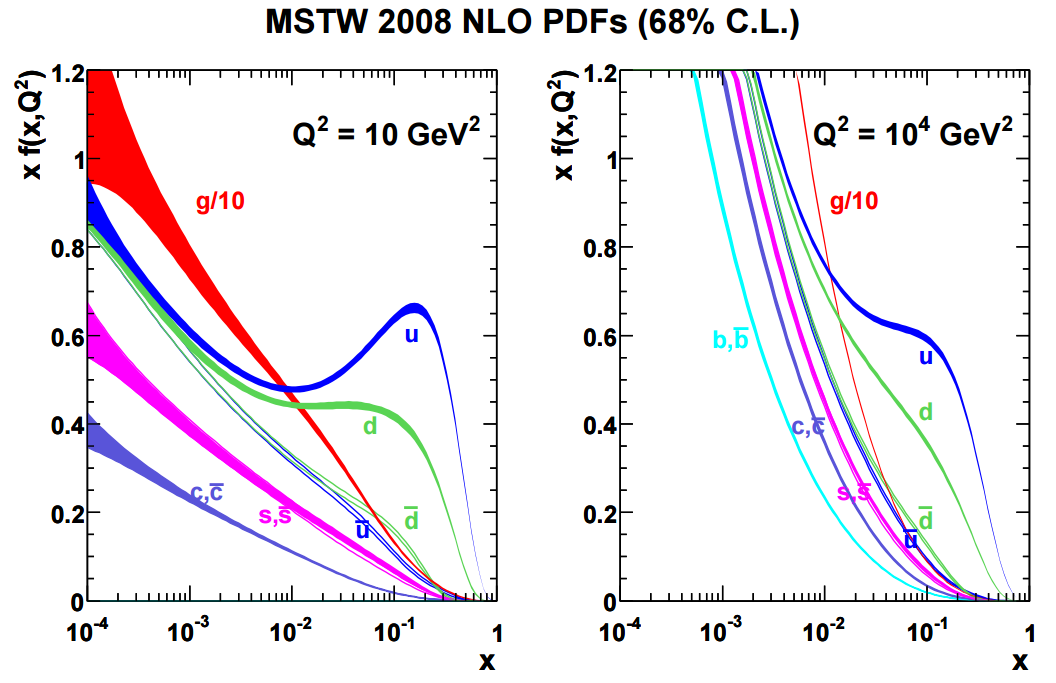
\includegraphics[width = 6 cm]{plots/part1/chapter2/PDFs.png}
	\end{figure}
	
	\begin{itemize}
		\item \footnotesize Hadrons made of partonic objects $\longrightarrow$ non perturbative physics
		\item \footnotesize Interactions take place only at partonic level
	\end{itemize}
	
	{\color{blue} \footnotesize Parton Distribution Functions: probability distribution of finding a particular parton \\ (u, d, ..., g) carrying a fraction x of the proton's momentum}

\end{frame}

% Parton densities
\begin{frame}
	
	\frametitle{QCD and collider physics}
	\framesubtitle{Parton densities}
	
	\begin{figure}
		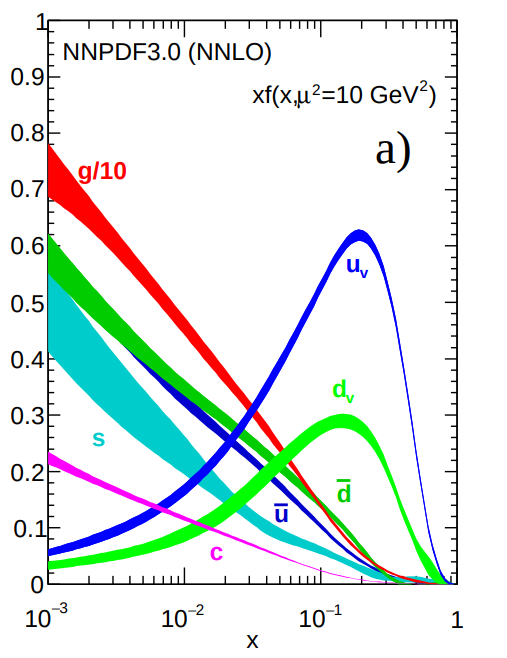
\includegraphics[width = 3 cm]{plots/part1/chapter2/PDF.png}
	\end{figure}
	
	\begin{itemize}
		\item \footnotesize Each parton has a different PDF $\longrightarrow$ ${\color{blue}u(x)}, {\color{green}d(x)}, ..., {\color{red}g(x)}$
		\item \footnotesize PDFs can not predicted and yet can not measured $\longrightarrow$ {\color{blue}extracted} from data
		\item \footnotesize The N$^{3}$PDF project: ML for PDFs determination
	\end{itemize}

\end{frame}

% Partonic cross section and pQCD
\begin{frame}
	
	\frametitle{QCD and collider physics}
	\framesubtitle{Partonic cross section and pQCD}
	
	\begin{columns}
	
	\column{0.45\textwidth}
	
	\begin{itemize}
		\item \footnotesize Born cross section is the leading-order (LO) term of the perturbative series
		\item \footnotesize $\sigma^{(1)}, \sigma^{(2)}, \sigma^{(3)}$ are the NLO, NNLO, N3LO corrections
	\end{itemize}
	
	\column{0.45\textwidth}
	\begin{figure}[!htb]
		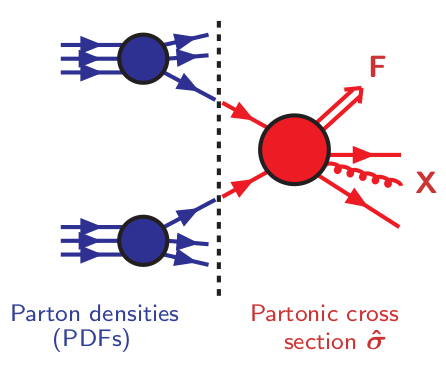
\includegraphics[width = 5 cm]{plots/part1/chapter2/factorization_3.png}
	\end{figure}
	
	\end{columns}
	
	\begin{equation}
		\hat{\sigma} = \sigma^{\texttt{Born}} \Big( 1 +
		\alpha_{s} \sigma^{(1)} + 
		\alpha_{s}^{2} \sigma^{(2)} + 
		\alpha_{s}^{3} \sigma^{(3)} + ... \Big) \nonumber
	\end{equation}
	
	\footnotesize Lower order predictions strongly depend on the auxiliary / unphysical scales \\ {\color{red}Need higher order corrections to increase theoretical accuracy!}

\end{frame}

% LHC physics
\begin{frame}
	
	\frametitle{QCD and collider physics}
	\framesubtitle{LHC phenomenology}
	
	\footnotesize Predictions made by the Standard Model
	
	\begin{itemize}
		\item \footnotesize Eight gluons and three generations of quarks, described by the SU(3) gauge group, mixing angles described by CKM matrix
		\item \footnotesize Three generations of charged leptons and three generations of massive neutrinos mixing angles described by PMNS matrix
		\item \footnotesize The photon and the massive $W^{\pm}$ and $Z$ bosons
		\item \footnotesize A scalar Higgs boson, responsible for the electroweak symmetry breaking 
	\end{itemize}

\end{frame}

% LHC physics
\begin{frame}
	
	\frametitle{QCD and collider physics}
	\framesubtitle{LHC phenomenology}
	
	\begin{figure}
		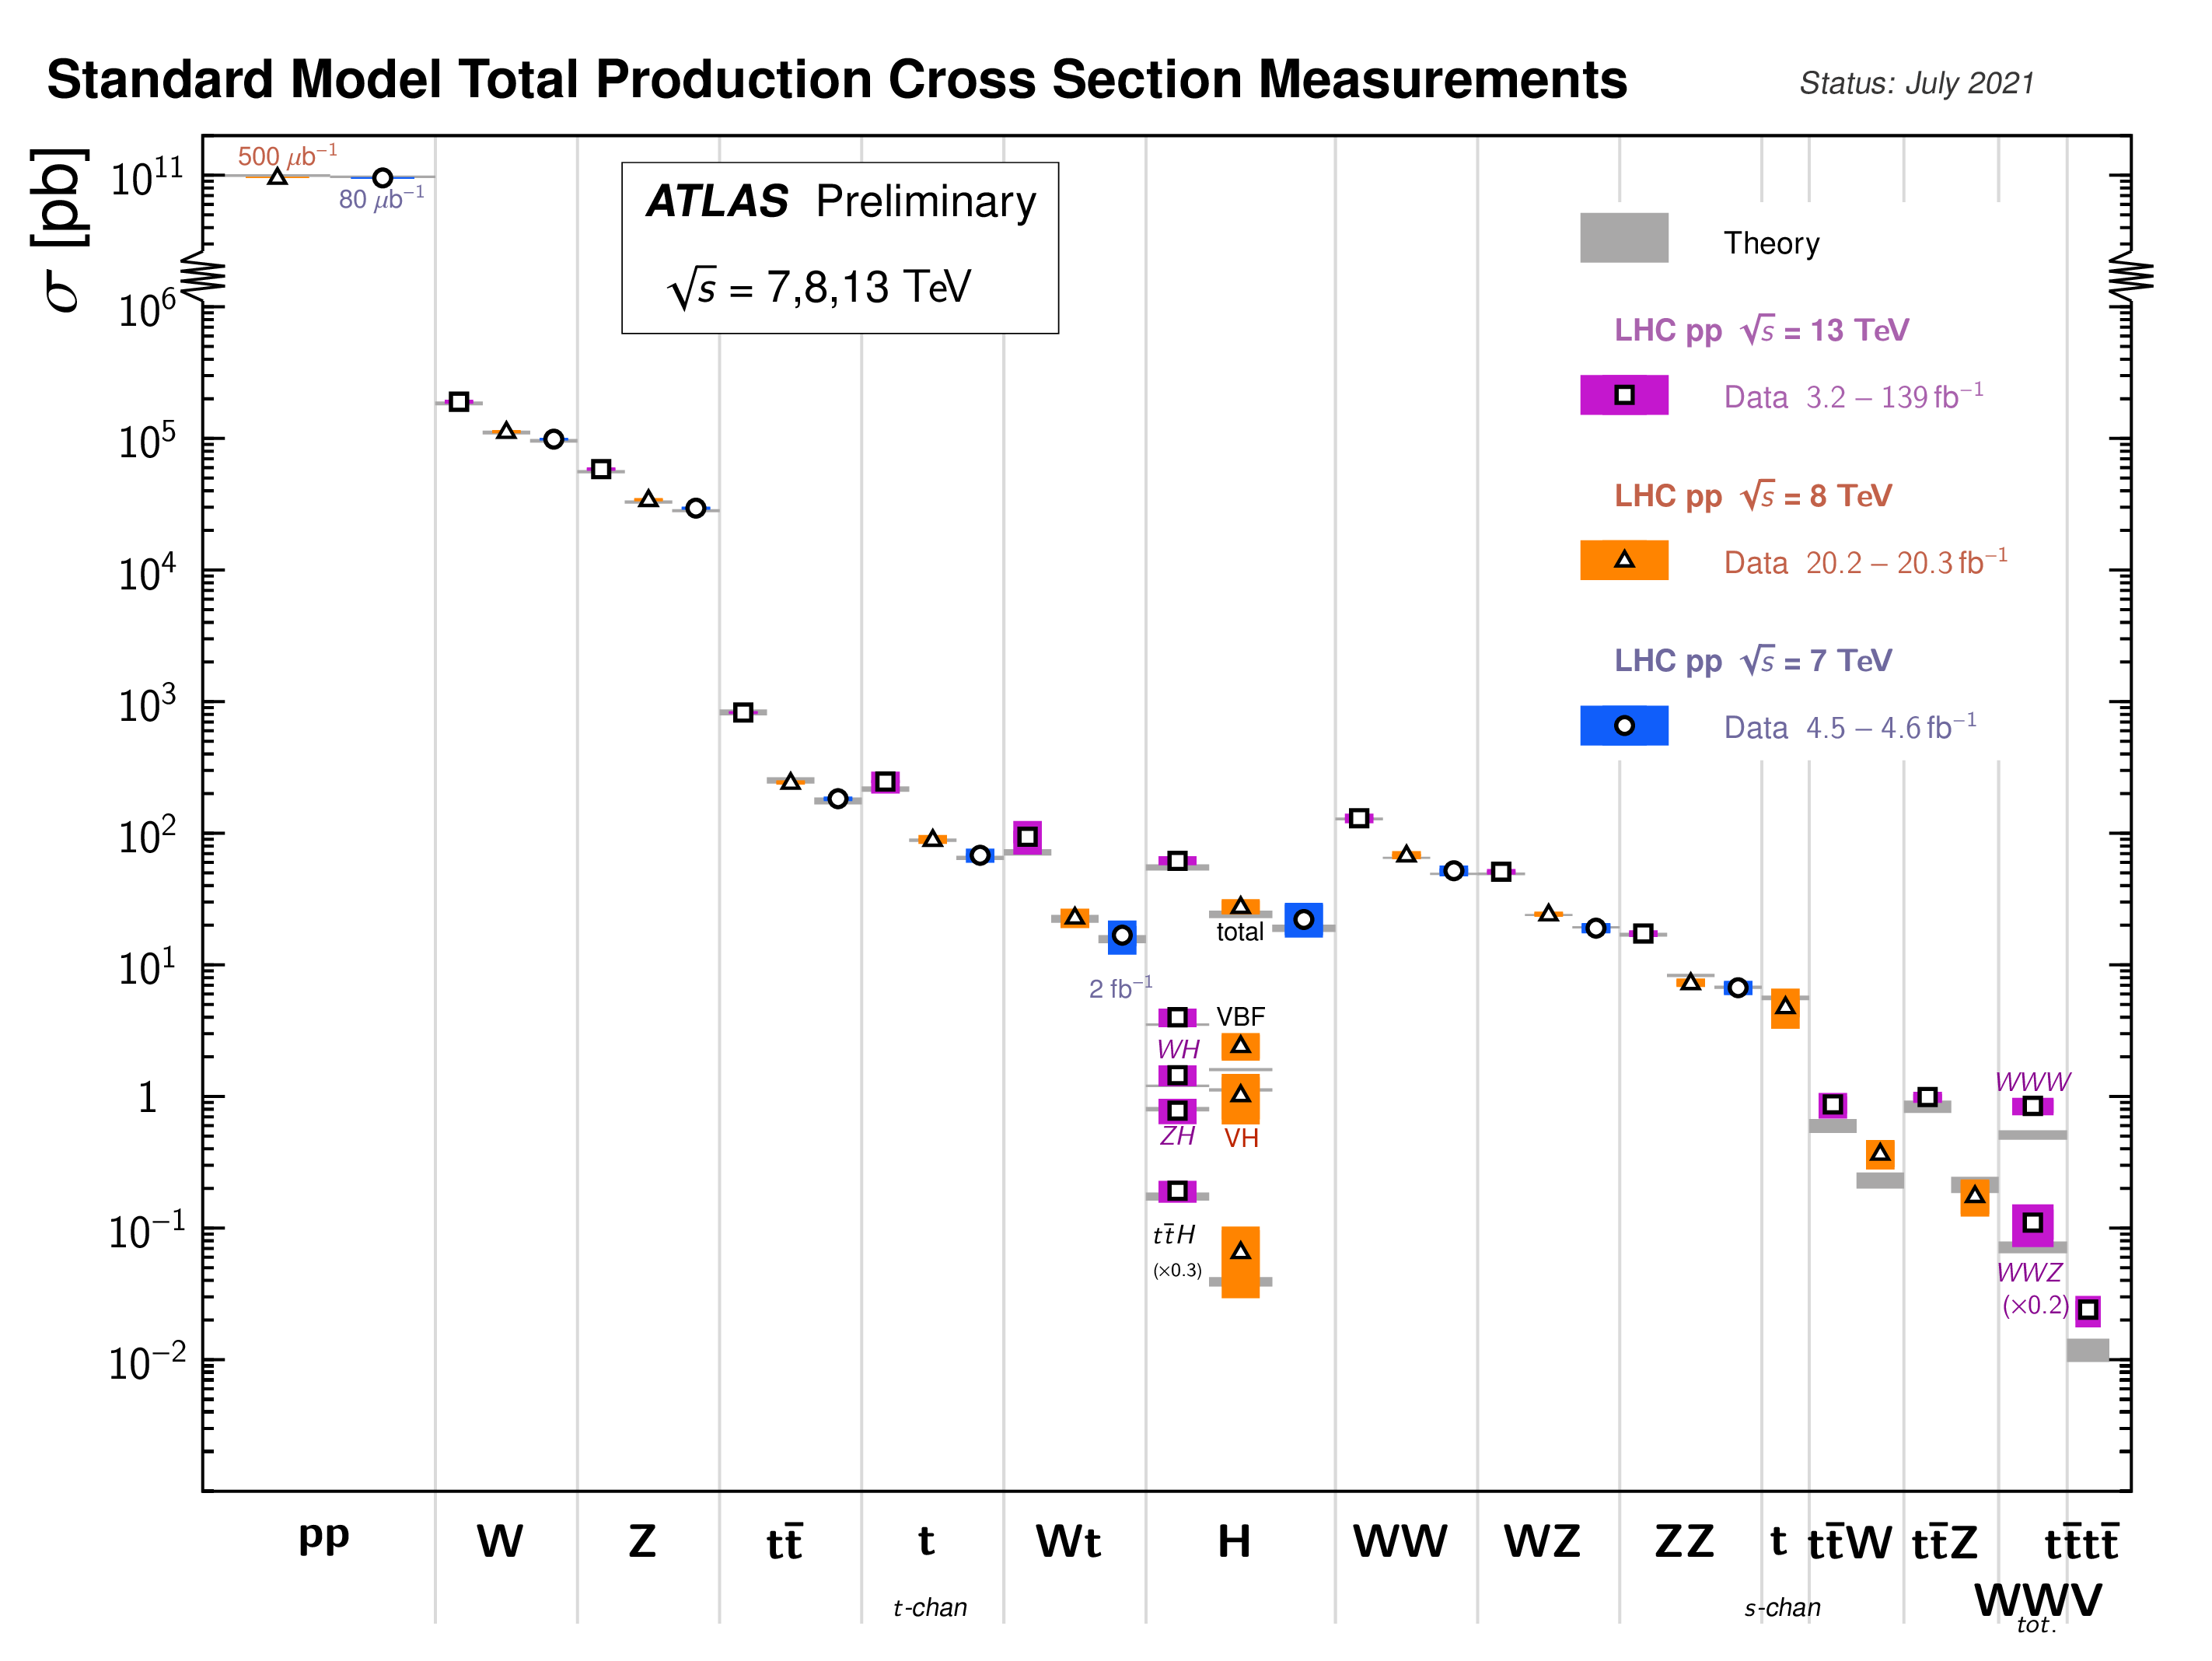
\includegraphics[width = 8.5 cm]{plots/part1/chapter3/lhc_measurements.png}
	\end{figure}

\end{frame}

% LHC physics
\begin{frame}
	
	\frametitle{QCD and collider physics}
	\framesubtitle{LHC phenomenology}
	
	\footnotesize Main processes studied at the LHC
	
	\begin{itemize}
		\item \footnotesize Deep inelastic scattering
		\item \footnotesize Drell-Yan lepton pair production
		\item \footnotesize Higgs boson production through gluon fusion
	\end{itemize}

\end{frame}

%
% Part 2 .................................................................................
% All order resummation ..................................................................
%

% Dealing with divergences
\begin{frame}

	\center{\color{blue}Part II \\ All order resummation}

\end{frame}

% The need for resummation
\begin{frame}
	
	\frametitle{Resummation in QCD}
	\framesubtitle{The need for resummation}

\end{frame}

% Higher order corrections
\begin{frame}

	\frametitle{Resummation in QCD}
	\framesubtitle{Higher order corrections}
	\begin{columns}
	
	\column{0.5\textwidth}
	
	\begin{enumerate}
		\item \footnotesize Calculation of higher order corrections is {\color{red}not an easy task} due to {\color{red} infrared (IR) soft and collinear singularities}
		\item \footnotesize Final state singularities {\color{blue}cancel} by combining real and virtual contributions
		\item \footnotesize Initial state collinear singularities {\color{blue}factorized} inside the PDFs
	\end{enumerate}
	
	\column{0.45\textwidth}
	\begin{figure}[!htb]
		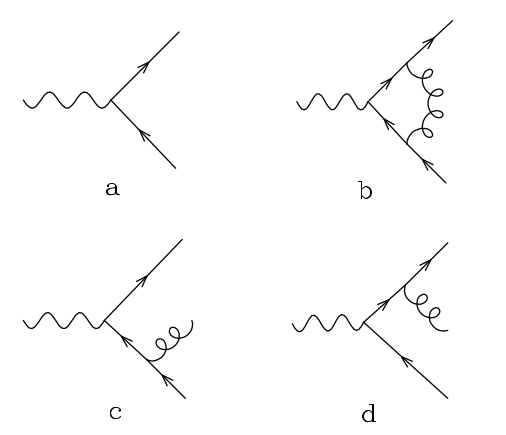
\includegraphics[width = \linewidth]{plots/part2/qcd_corrections.png}
	\end{figure}
	
	\end{columns}

\end{frame}

% qT resummation I
\begin{frame}

	\frametitle{Resummation in QCD}
	\framesubtitle{$q_{\perp}$ resummation}
	
	\begin{columns}
	
		\column{0.55\textwidth}
		
		\center	\footnotesize Study the differential $q_{\perp}$ distribution \\
		\center	$h_{1}(p_{1}) + h_{2}(p_{2}) \longrightarrow F(M, {\color{red}q_{\perp}}) + X$
	
		\column{0.45\textwidth}
		
		\begin{figure}
			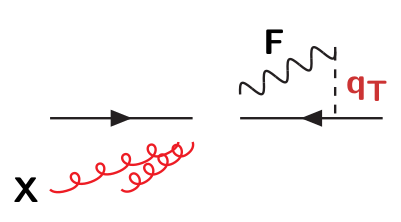
\includegraphics[width = 4cm]{plots/part2/qT_diagram.png}
		\end{figure}

	\end{columns}

	\footnotesize 
	$\int_{0}^{Q_{\perp}^{2}} \; dq_{\perp}^{2} \frac{d\hat{\sigma}}{dq_{\perp}^{2}} \sim c_{0} + \alpha_{s}(c_{12}L^{2} + c_{11}L + c_{10}) + ..., \textrm{\quad where \quad} L = \ln (q_{\perp} / M^{2})$

	\begin{figure}
		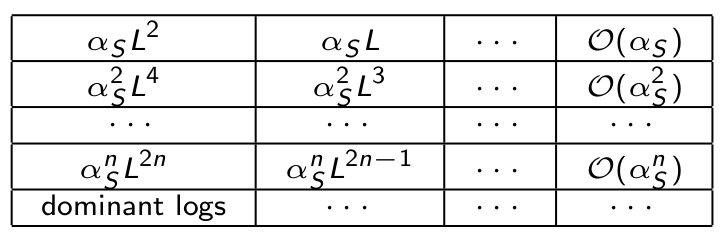
\includegraphics[width = 7.5cm]{plots/part2/qT_logs_table.png}
	\end{figure}

	\footnotesize Truncated fixed order predictions $\rightarrow$ {\color{red}enhanced $\alpha_{s}^{n}\ln^{m}(M^{2}/q_{\perp}^{2})$ appear}

\end{frame}

% Resummation in QCD II
\begin{frame}

	\frametitle{Resummation in QCD}
	\framesubtitle{$q_{\perp}$ resummation}

	\footnotesize Separate partonic $q_{\perp}$ distribution as follows
	
	\begin{equation}
		\frac{d\hat{\sigma}_{ab}}{dq_{\perp}^{2}} =
		\Bigg[ \frac{d\hat{\sigma}^{\textrm{(res.)}}_{ab}}{dq_{\perp}^{2}} \Bigg]_{\textrm{l.a.}} + 
		\Bigg[ \frac{d\hat{\sigma}^{\textrm{(fin.)}}_{ab}}{dq_{\perp}^{2}} \Bigg]_{\textrm{f.o.}} \textrm{\quad, \quad such that} \nonumber
	\end{equation}

	\begin{align}
		\int_{0}^{q_{\perp}^{2}} dq_{\perp}^{2} \frac{d\hat{\sigma}^{\textrm{(res.)}}_{ab}}{dq_{\perp}^{2}} \sim & \sum \alpha_{s}^{n} \log^{m} \frac{M^{2}}{q_{\perp}^{2}} \textrm{\quad for \quad} q_{\perp} \rightarrow 0 \nonumber \\
		\lim_{q_{\perp} \rightarrow 0}\int_{0}^{q_{\perp}^{2}} dq_{\perp}^{2} \frac{d\hat{\sigma}^{\textrm{(fin.)}}_{ab}}{dq_{\perp}^{2}} &= 0 \nonumber 
	\end{align}

	\footnotesize Resummed and finite components can be matched (LL+LO, NLL+NLO,\\ NNLO+NNLL, ...) to have uniform accuracy in a wide range of $q_{\perp}$
\end{frame}

% qT resummation III
\begin{frame}

	\frametitle{Resummation in QCD}
	\framesubtitle{$q_{\perp}$ resummation}
	
	\footnotesize Resummation holds in impact parameter space $b$
	\begin{equation}
		\frac{d\hat{\sigma}_{ab}^{\textrm{(res.)}}}{dq_{\perp}^{2}} = \frac{M^{2}}{\hat{s}} \int db \; \frac{b}{2} \; J_{0}(b q_{\perp}) \; {\color{red} \mathcal{W}_{ab}(b, M)} \nonumber
	\end{equation}
	
	\footnotesize 
	with ${\color{red}\mathcal{W}_{ab}}$ also expressed in Mellin space (with respect to $z = M^{2}/\hat{s}$)
	\begin{equation}
		{\color{red} \mathcal{W}_{N}(b, M) = \mathcal{H}_{N}(\alpha_{s}) \times \exp\{\mathcal{G}_{N}(\alpha_{s}, L)\}} \quad\textrm{being}\quad L \equiv \log(M^{2}b^{2}) \nonumber
	\end{equation}

	\begin{itemize}
		\item Large logarithms exponentiated in the universal Sudakov form factor {\color{red}$\mathcal{G}_{N}(\alpha_{s}, L)$}
		\item Constant (b-independent) terms factorized in the process dependent hard factor {\color{red}$\mathcal{H}_{N}(\alpha_{s})$}
	\end{itemize}

	
\end{frame}

%
% Part 3 .................................................................................
% HTurbo numerical implementation ........................................................
%

% Part 3
\begin{frame}

	\center{\color{blue}Part III \\ HTurbo numerical implementation}

\end{frame}

% Need for fast numerical implementations
\begin{frame}
	
	\frametitle{HqT and HRes}
	\framesubtitle{Need for fast numerical implementations}

\end{frame}

% HqT and HRes
\begin{frame}

	\frametitle{HqT and HRes}
	\framesubtitle{Predictions for Higgs $q_{\perp}$ distribution}
	
	\begin{columns}
		
		\column{0.5\textwidth}
			
		\begin{itemize}
			\item $q_{\perp}$ resummation implemented in numerical codes HqT and HRes {\color{blue}[Catani, de Florian, Ferrera, Grazzini, Tommasini]} 
			\item Higher order accuracy require {\color{red}high computation times}
			\item Codes producing fast and accurate predictions are needed for precision era of the LHC
		\end{itemize}

		\column{0.55\textwidth}
	
		\begin{figure}
			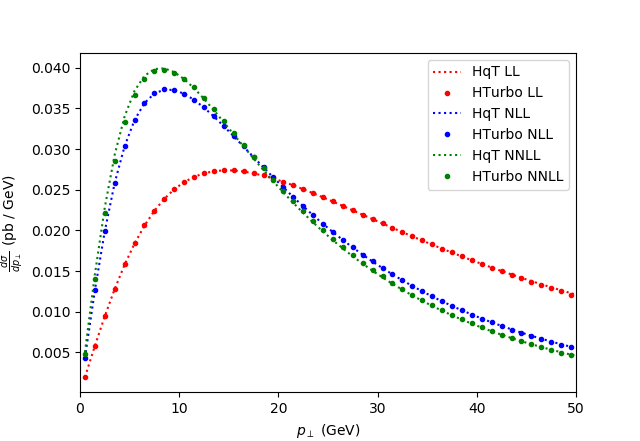
\includegraphics[width = 7 cm]{plots/part3/chapter6/higgs_qt_all.png}
		\end{figure}		
			
	\end{columns}

\end{frame}

% DYturbo I
\begin{frame}

	\frametitle{HTurbo}
	\framesubtitle{Starting point DYTurbo}

	Numerical code \textbf{DYTurbo} {\color{blue}[Camarda et al.]} ref. at {\color{blue} \href{https://arxiv.org/abs/1910.07049}{1910.07049}}, fast and precise $q_{\perp}$ resummation and several improvements for Drell-Yan ($h_{1}h_{2} \rightarrow V + X \rightarrow l^{+}l^{-} + X$) 
	
	\begin{itemize}
		\item {\color{red}First goal}: set up a numerical code for Higgs boson production starting from  \textbf{DYTurbo}
		\item Set LO amplitude $gg \rightarrow H$
		\item Set Sudakov and Hard coefficients for Higgs production
		\item Compare with \textbf{HRes} and \textbf{HqT}
	\end{itemize}

	\vspace{0.5 cm}

	{\color{red}Final goal}: extend theoretical accuracy up to N$^{3}$LL+N$^{3}$LO

\end{frame}

% DYturbo II
\begin{frame}

	\frametitle{HTurbo}
	\framesubtitle{Starting point DYTurbo}

	Both Sudakov factor $\mathcal{G}_{N}$ and hard coefficient $\mathcal{H}_{N}$ can be expanded as perturbative series in $\alpha_{s}$
	\begin{align}
		\mathcal{G}_{N}(\alpha_{s}, L) &= L\;g^{(1)}(\alpha_{s}L) + g^{(2)}(\alpha_{s}L) + \frac{\alpha_{s}}{\pi}g^{(3)}(\alpha_{s}L) + ... \nonumber \\
		\mathcal{H}_{N}(\alpha_{s}) &= 1 + \alpha_{s}\mathcal{H}^{(1)} + \alpha_{s}^{2}\mathcal{H}^{(2)} + ...  \nonumber
	\end{align}
	
	For each new order implement a factor of $\mathcal{G}_{N}$ and Hard $\mathcal{H}_{N}$
	
	\begin{columns}
		
		\column{0.45\textwidth}

		\begin{align}
			&\textrm{LL} (\sim \alpha_{s}^{n}L^{n+1}): g^{(1)}, \hat{\sigma}^{(0)} \nonumber \\
			&\textrm{NLL} (\sim \alpha_{s}^{n}L^{n}): g^{(2)}, \mathcal{H}^{(1)} \nonumber \\
			&\textrm{NNLL} (\sim \alpha_{s}^{n}L^{n-1}): g^{(3)}, \mathcal{H}^{(2)} \nonumber
		\end{align}
	
		\column{0.45\textwidth}
		
		Start by building predictions up to NNLO+NNLL, then add {\color{blue}N$^{3}$LO+N$^{3}$LL}
		
	\end{columns}

\end{frame}

% DYturbo II
\begin{frame}

	\frametitle{HTurbo}
	\framesubtitle{Code optimization}
	
	Reimplementation of \textbf{HqT} and \textbf{HRes} for $q_{T}$-resummation
	\begin{itemize}
		\item \textbf{C++} structure with \textbf{Fortran} interfaces $\rightarrow$ Multi-threading
		\item Optimization in the integration routines / integral transforms 
		\begin{itemize}
			\item Factorize boson and decay kinematics
			\item Gauss-Legendre quadrature rules (1-dim.)
			\item Vegas/Cuhre through \textbf{Cuba} (multi-dim.)
		\end{itemize}
	\end{itemize}
	
	\vspace{0.5cm}
	
	Comparison \textbf{HRes} and \textbf{HTurbo} - speed performance \\
	\center
	\begin{tabular}{ | c | c | c | }
		\hline
		Predictions & \textbf{HRes} & \textbf{HTurbo} \\ 
		\hline
		resummed NNLL & 10h & 10' \\
		\hline
		combined NNLO+NNLL & 20h & 1h \\
		\hline
	\end{tabular}

	
\end{frame}

% Results - Benchmark HRes - NLL resummed
\begin{frame}
	
	\frametitle{Results}
	\framesubtitle{Comparison HTurbo and HRes - NLL resummed}
	
	\begin{columns}
		
		\column{0.5\textwidth}
		
		\begin{figure}
			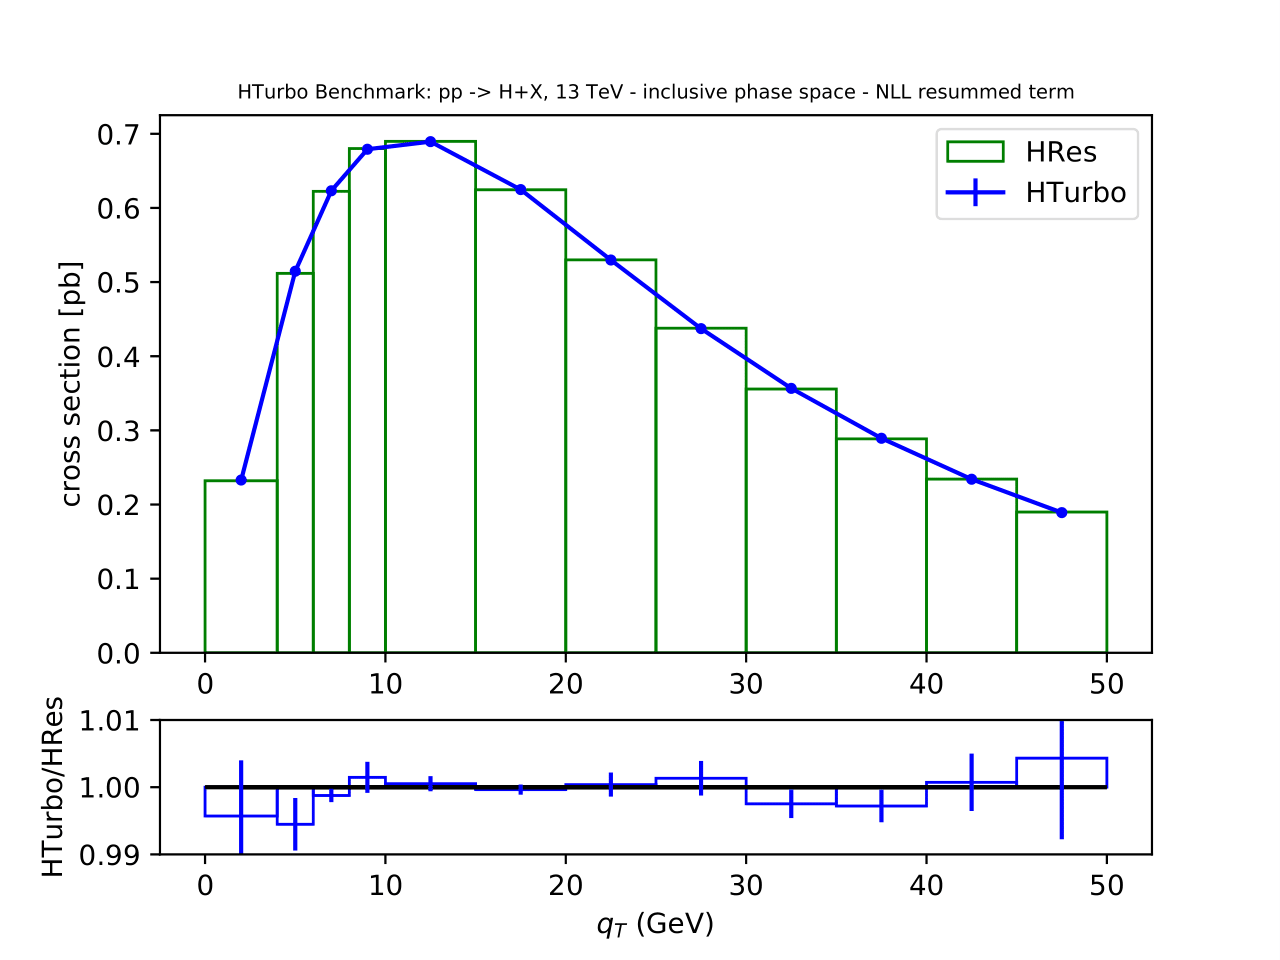
\includegraphics[width = 7cm]{plots/part3/chapter6/nlo-res-1.png}
		\end{figure}
		
		\column{0.5\textwidth}
		
		\begin{figure}
			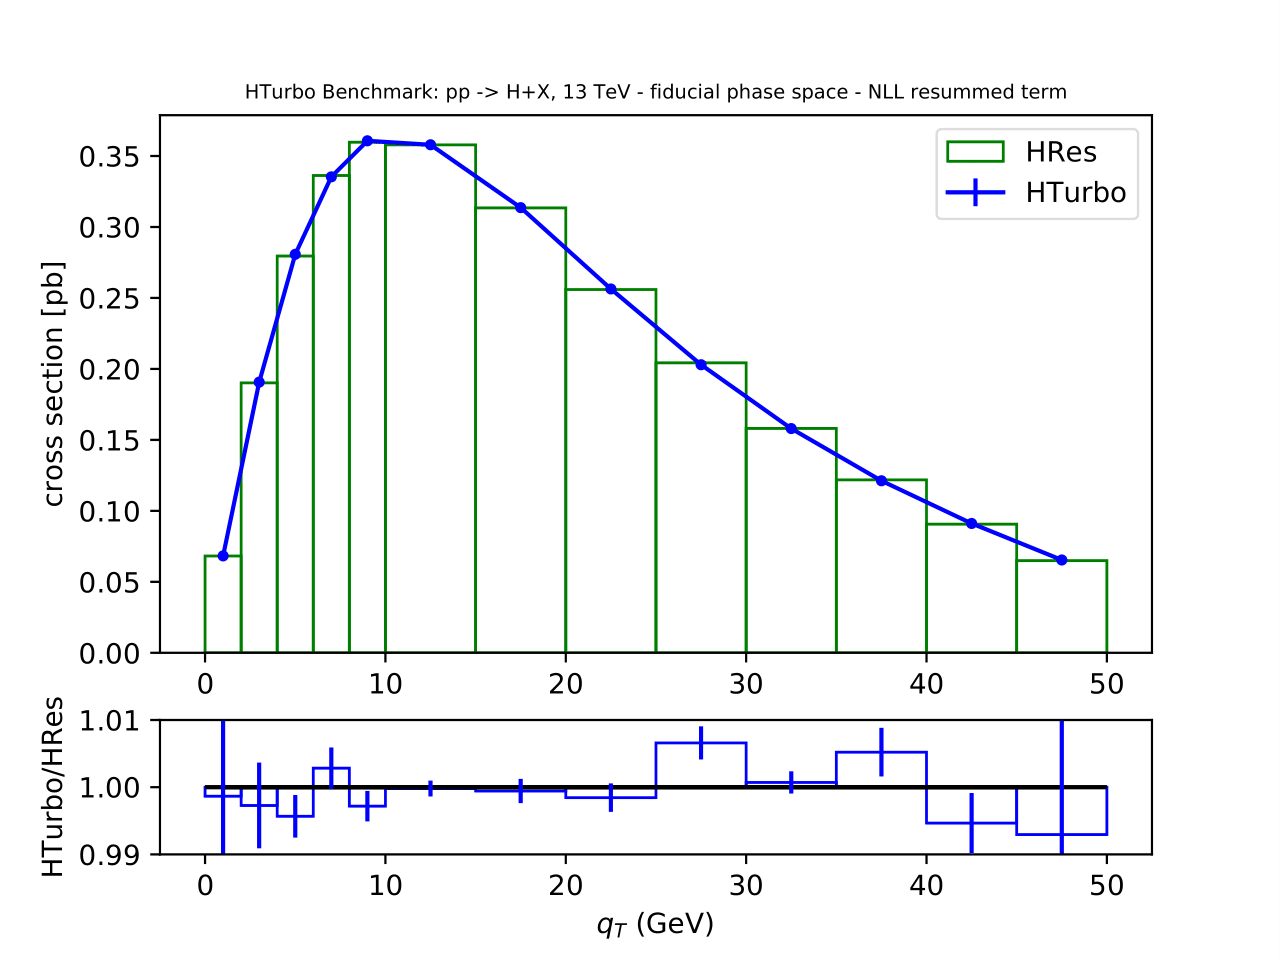
\includegraphics[width = 7cm]{plots/part3/chapter6/nlo-res-fid-1.png}
		\end{figure}
		
	\end{columns}
	
	\begin{itemize}
		\item \footnotesize Represent full (LHS) and fiducial (RHS) phase space {\color{darkgreen}$\checkmark$} 
		\item \footnotesize Excellent numerical agreement at NLL
	\end{itemize}

\end{frame}

% Results - Benchmark HRes - NNLL resummed
\begin{frame}
	
	\frametitle{Results}
	\framesubtitle{Comparison HTurbo and HRes - NNLL resummed}
	
	\begin{columns}
	
	\column{0.5\textwidth}
	
	\begin{figure}
		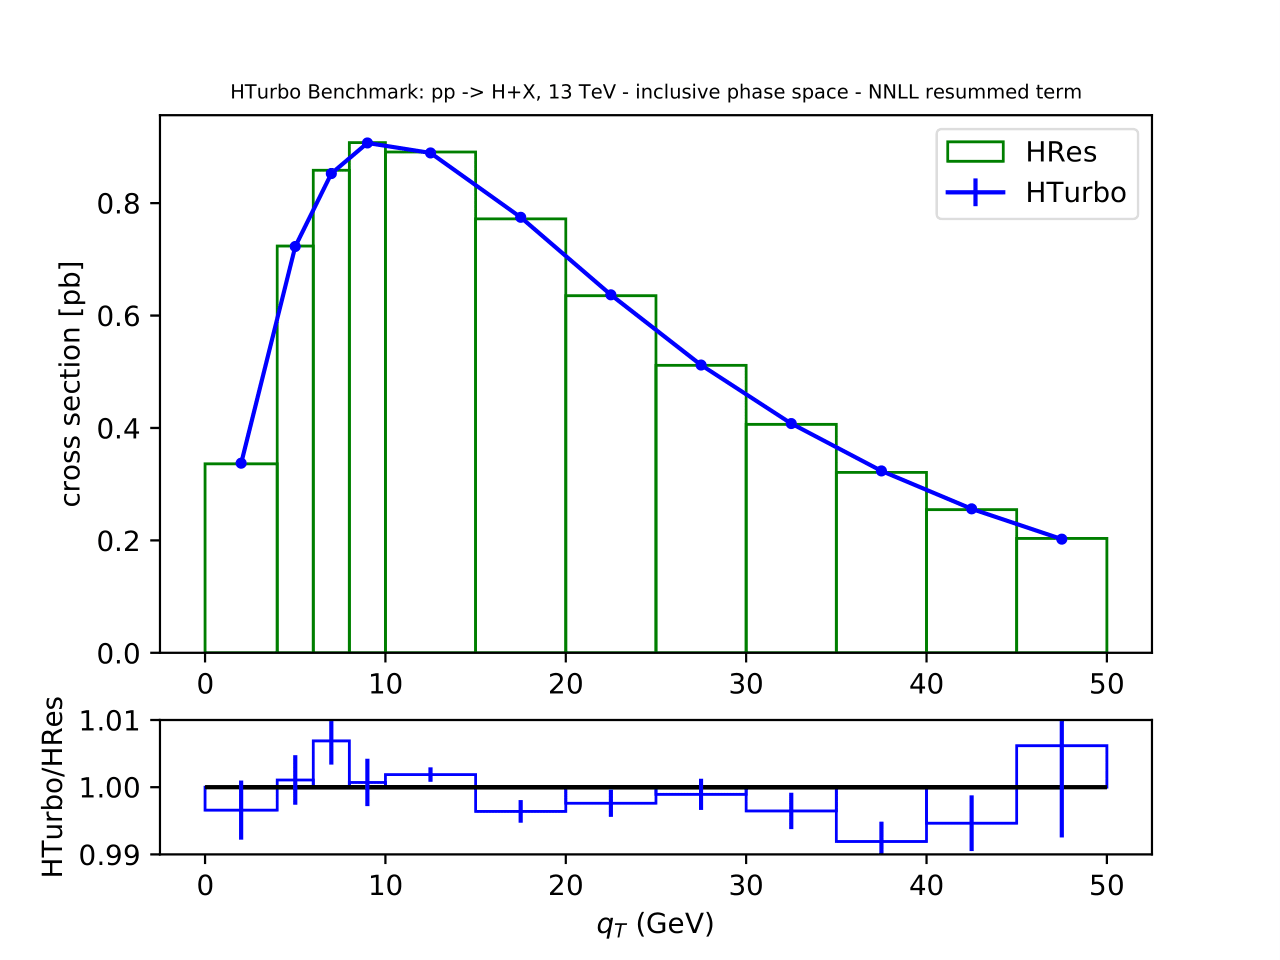
\includegraphics[width = 7cm]{plots/part3/chapter6/nnlo-res-1.png}
	\end{figure}
	
	\column{0.5\textwidth}
	
	\begin{figure}
		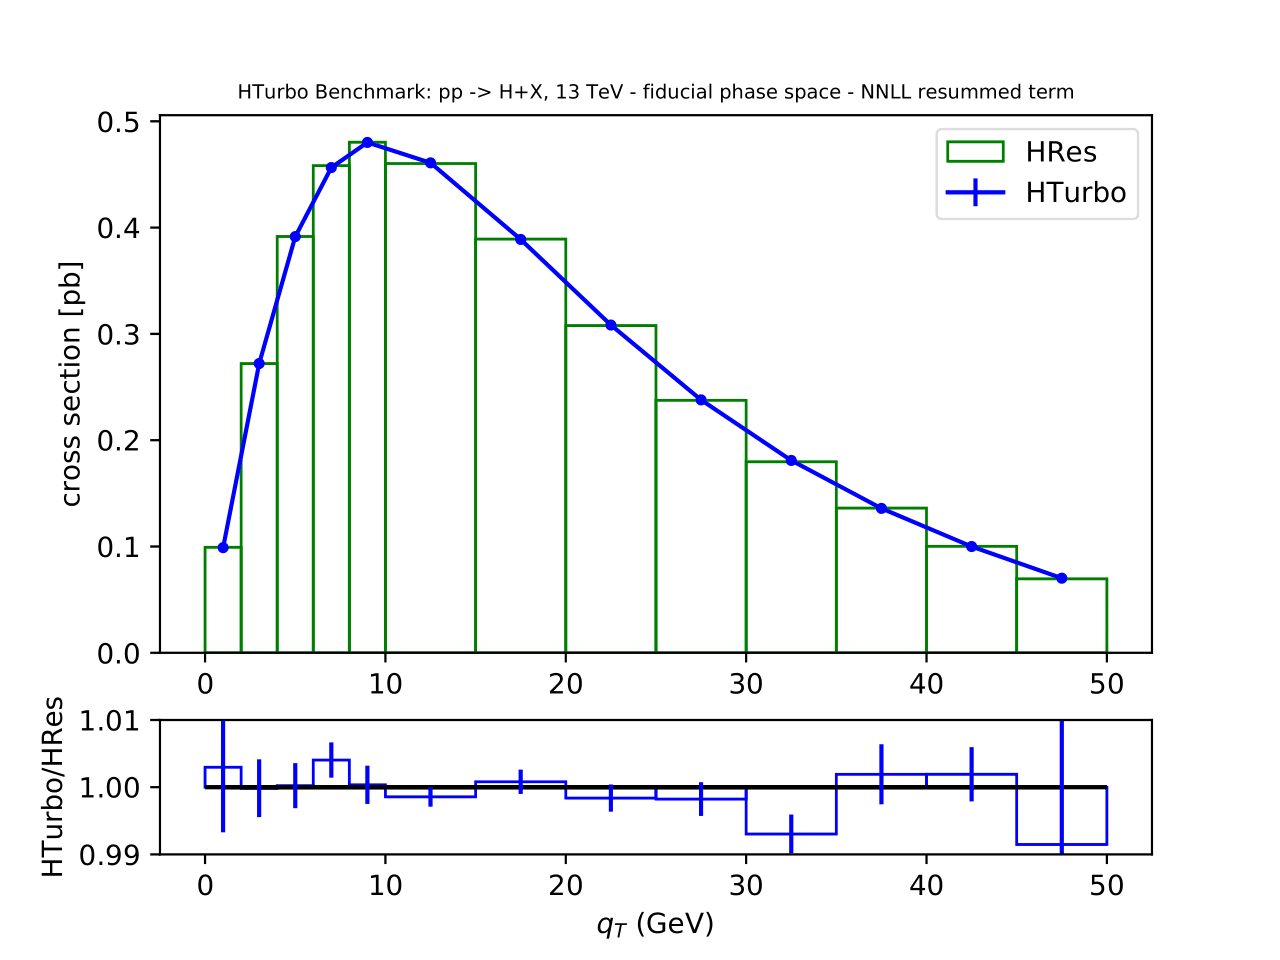
\includegraphics[width = 7cm]{plots/part3/chapter6/nnlo-res-fid-1.png}
	\end{figure}
	
	\end{columns}
	
	\begin{itemize}
	\item \footnotesize Represent full (LHS) and fiducial (RHS) phase space {\color{darkgreen}$\checkmark$} 
	\item \footnotesize Excellent numerical agreement at NNLL
	\end{itemize}

\end{frame}

% Results - Benchmark HRes - LO asymptotic
\begin{frame}
	
	\frametitle{Results}
	\framesubtitle{Comparison HTurbo and HRes - LO asymptotic}
	
	\begin{columns}
		
		\column{0.5\textwidth}
		
		\begin{figure}
			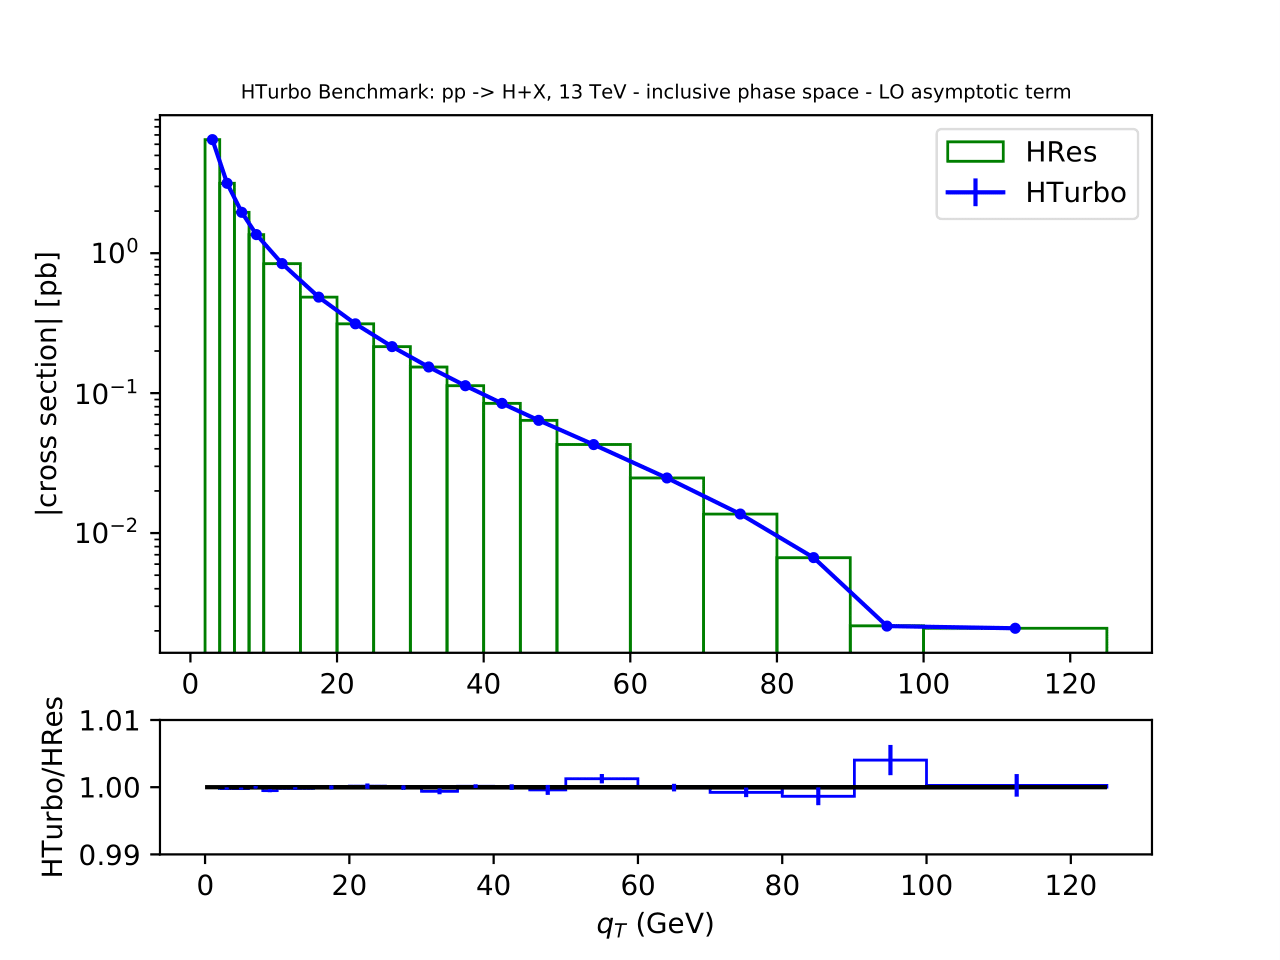
\includegraphics[width = 7cm]{plots/part3/chapter6/nlo-ct-1.png}
		\end{figure}
		
		\column{0.5\textwidth}
		
		\begin{figure}
			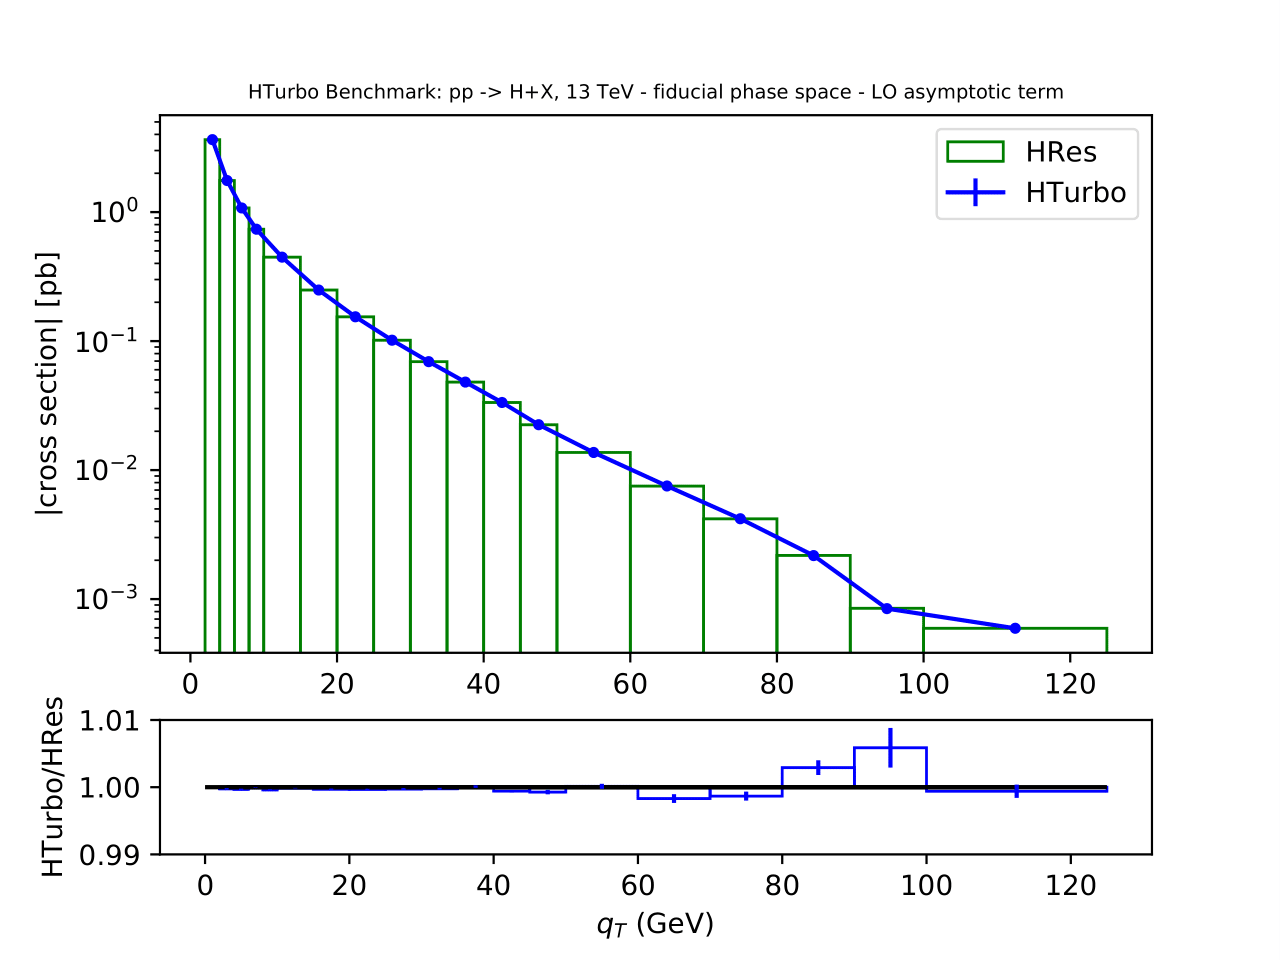
\includegraphics[width = 7cm]{plots/part3/chapter6/nlo-ct-fid-1.png}
		\end{figure}
		
	\end{columns}
	
	\begin{itemize}
		\item \footnotesize Represent full (LHS) and fiducial (RHS) phase space {\color{darkgreen}$\checkmark$} 
		\item \footnotesize Excellent numerical agreement at LO
	\end{itemize}

\end{frame}

% Results - Benchmark HRes - NLO asymptotic
\begin{frame}

\frametitle{Results}
\framesubtitle{Comparison HTurbo and HRes - NLO asymptotic}

	\begin{columns}
		
		\column{0.5\textwidth}
		
		\begin{figure}
			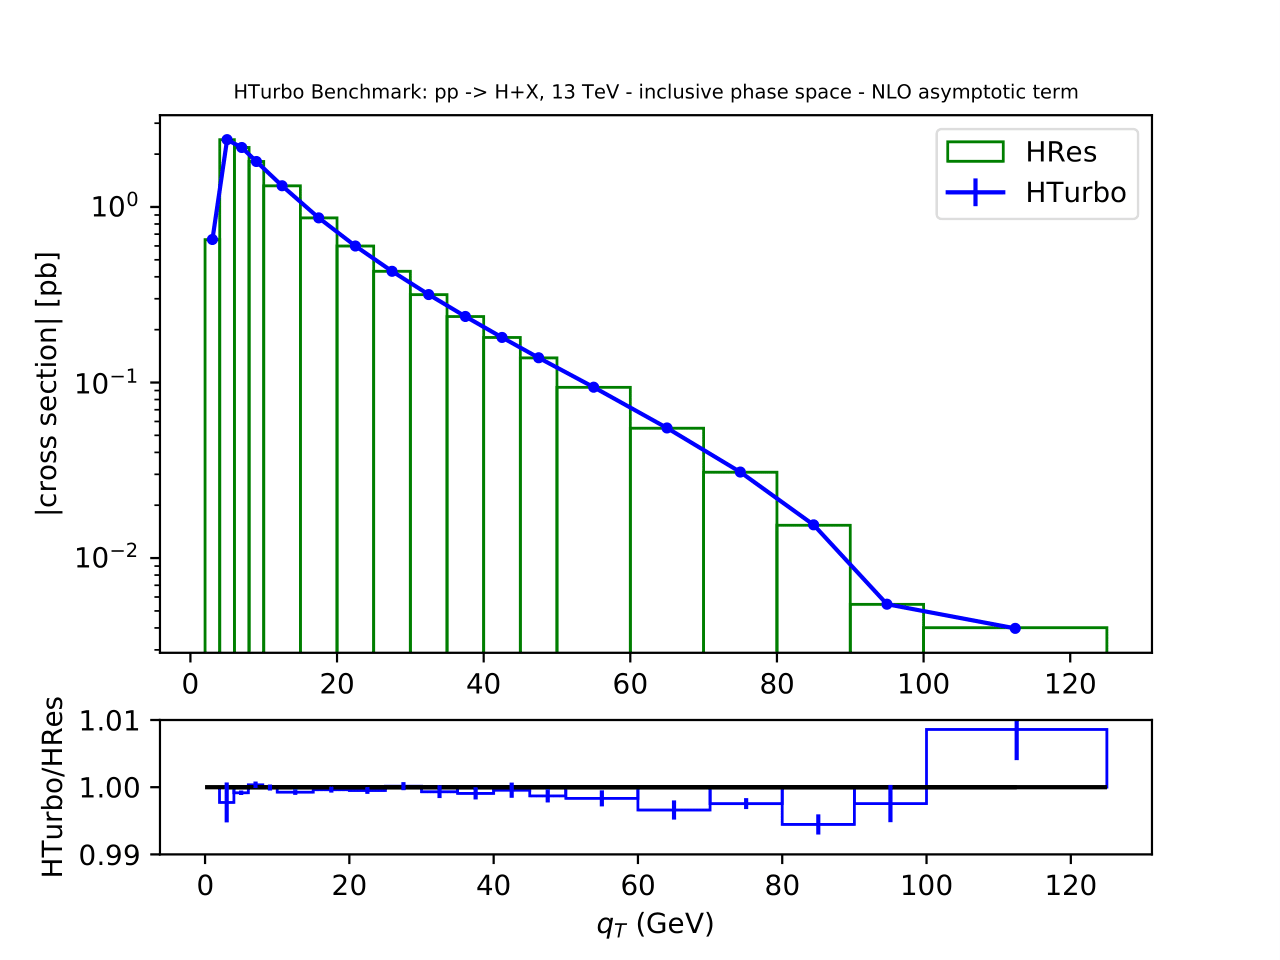
\includegraphics[width = 7cm]{plots/part3/chapter6/nnlo-ct-1.png}
		\end{figure}
		
		\column{0.5\textwidth}
		
		\begin{figure}
			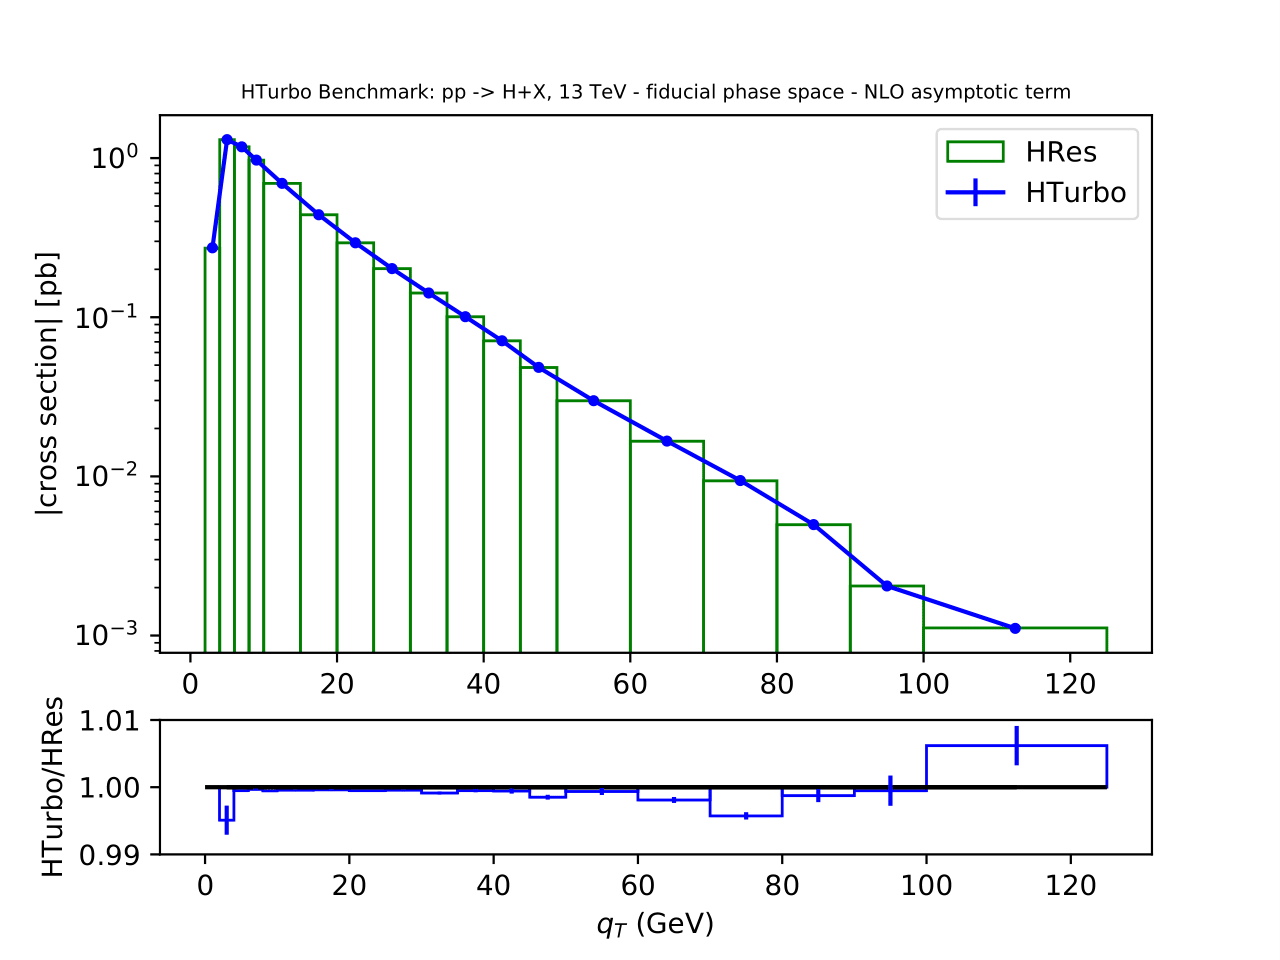
\includegraphics[width = 7cm]{plots/part3/chapter6/nnlo-ct-fid-1.png}
		\end{figure}
		
	\end{columns}
	
	\begin{itemize}
		\item \footnotesize Represent full (LHS) and fiducial (RHS) phase space {\color{darkgreen}$\checkmark$} 
		\item \footnotesize Excellent numerical agreement at NLO
	\end{itemize}

\end{frame}

% Results - Benchmark HRes - LO fixed-order
\begin{frame}

	\frametitle{Results}
	\framesubtitle{Comparison HTurbo and HRes - LO fixed-order}
	
	\begin{columns}
		
		\column{0.5\textwidth}
		
		\begin{figure}
			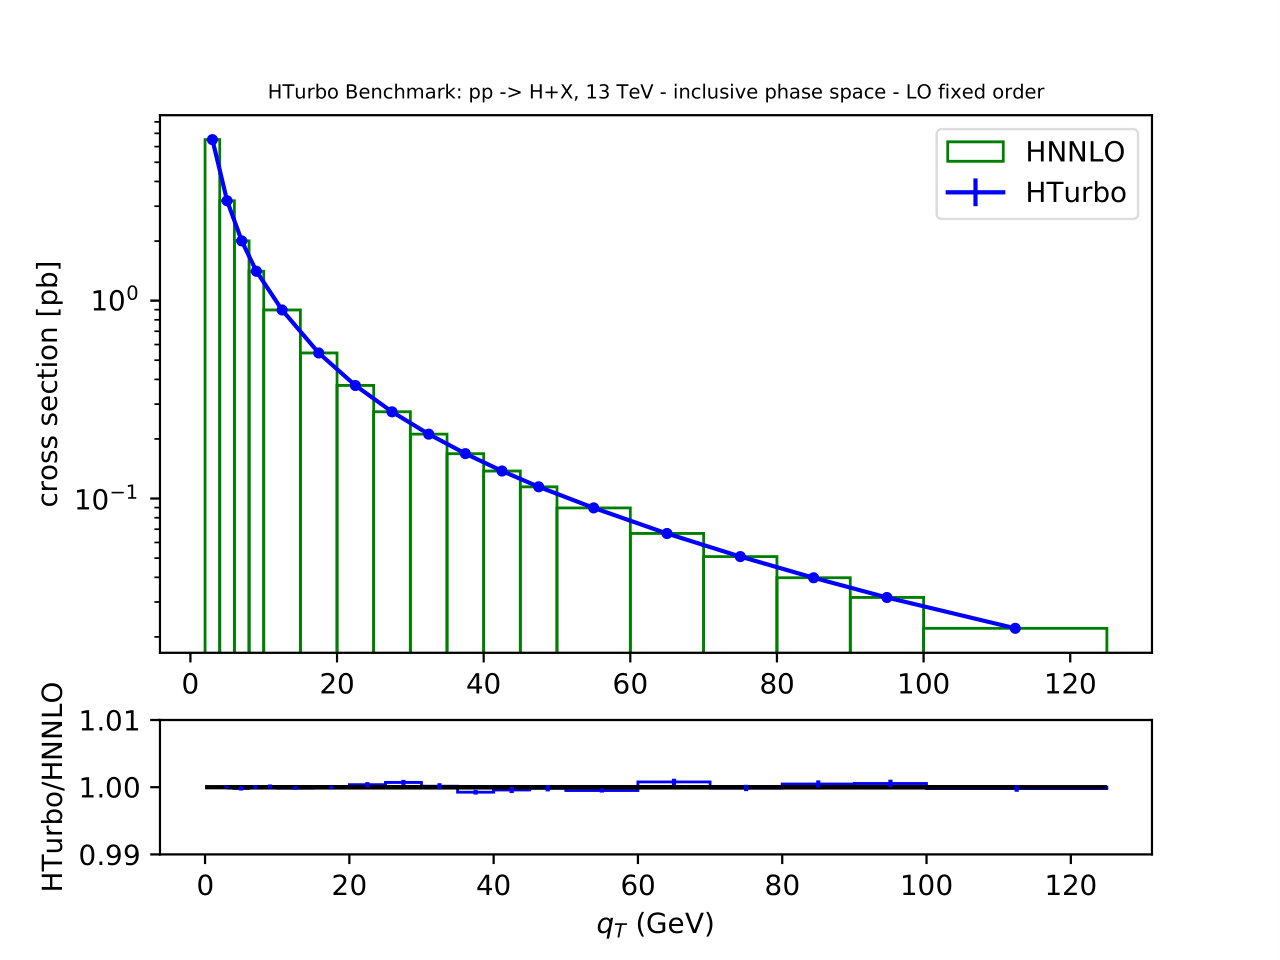
\includegraphics[width = 7cm]{plots/part3/chapter6/nlo-fo-1.png}
		\end{figure}
		
		\column{0.5\textwidth}
		
		\begin{figure}
			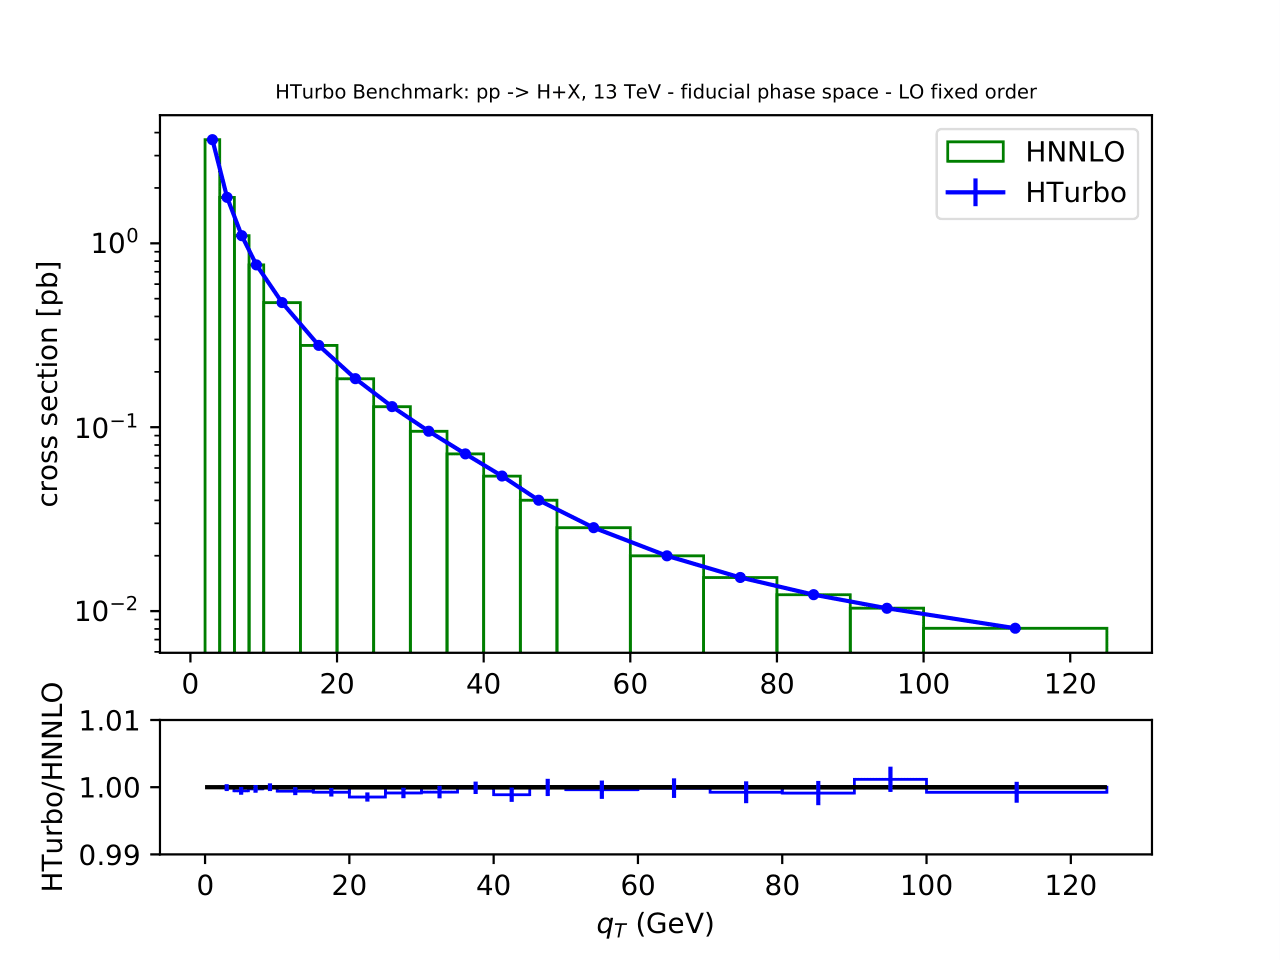
\includegraphics[width = 7cm]{plots/part3/chapter6/nlo-fo-fid-1.png}
		\end{figure}
		
	\end{columns}
	
	\begin{itemize}
		\item \footnotesize Represent full (LHS) and fiducial (RHS) phase space {\color{darkgreen}$\checkmark$} 
		\item \footnotesize Excellent numerical agreement at LO
	\end{itemize}

\end{frame}

% Results - Benchmark HRes - LO fixed-order
\begin{frame}
	
	\frametitle{Results}
	\framesubtitle{Comparison HTurbo and HRes - NLO fixed-order}
	
	\begin{columns}
		
		\column{0.5\textwidth}
		
		\begin{figure}
			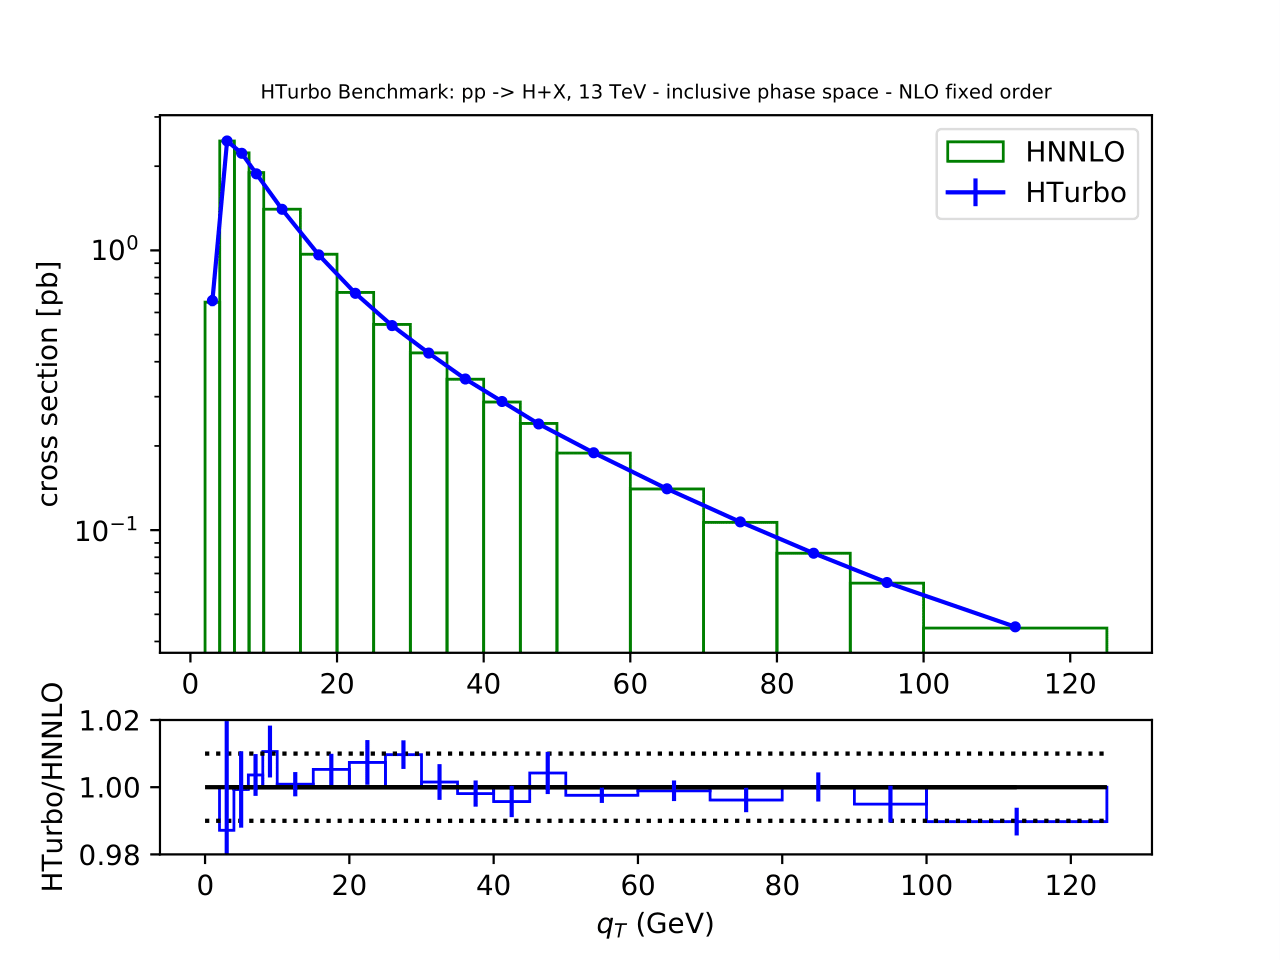
\includegraphics[width = 7cm]{plots/part3/chapter6/nnlo-fo-1.png}
		\end{figure}
		
		\column{0.5\textwidth}
		
		\begin{figure}
			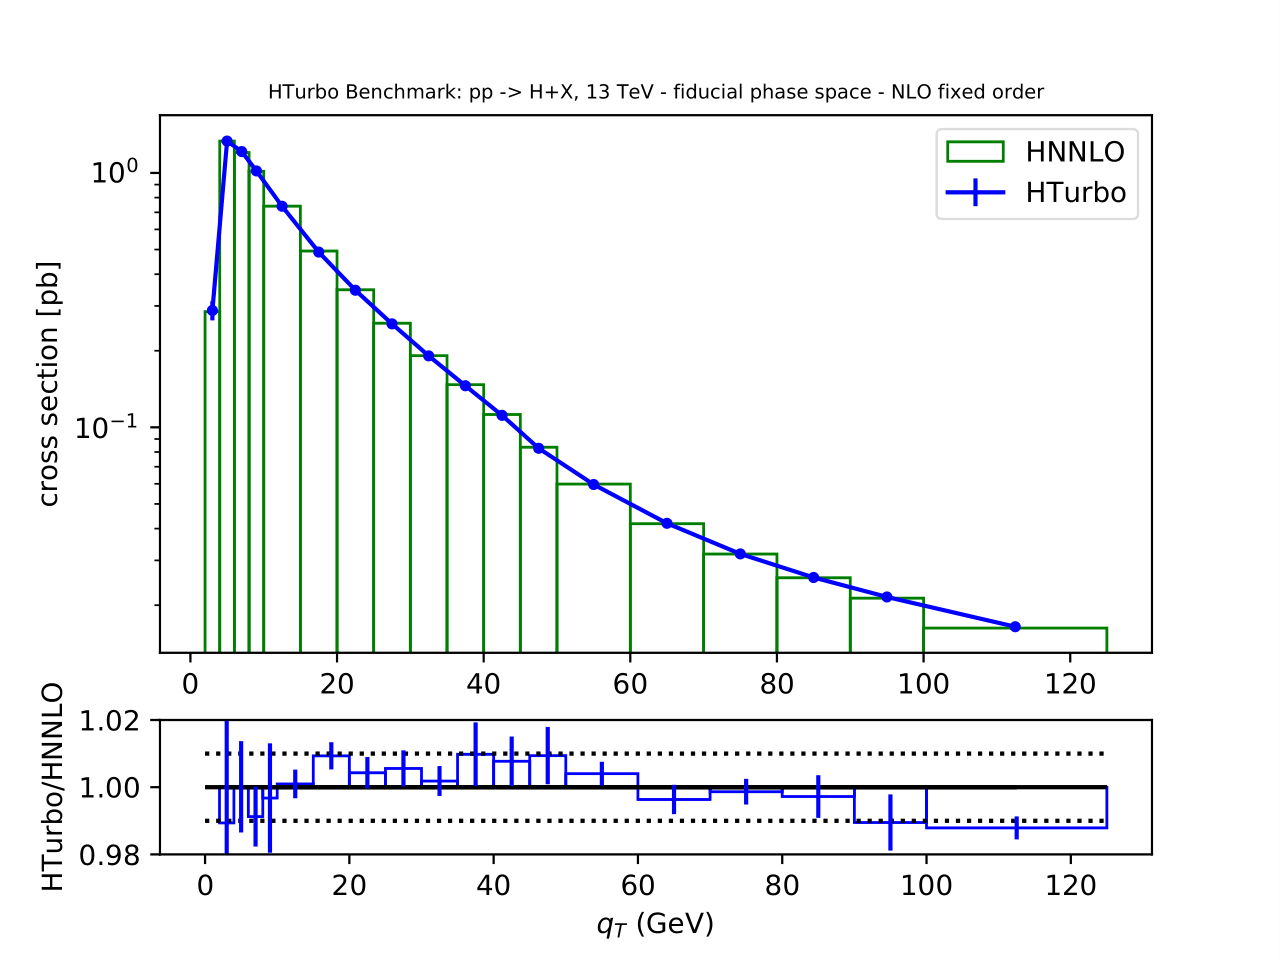
\includegraphics[width = 7cm]{plots/part3/chapter6/nnlo-fo-fid-1.png}
		\end{figure}
		
	\end{columns}
	
	\begin{itemize}
		\item \footnotesize Represent full (LHS) and fiducial (RHS) phase space {\color{darkgreen}$\checkmark$} 
		\item \footnotesize Excellent numerical agreement at NLO
	\end{itemize}

\end{frame}

% Summary $\&$ Conclusions
\begin{frame}
	
	\frametitle{Summary $\&$ Conclusions}
	
	\vspace{2.0 cm}
	
	\begin{enumerate}
		\item \footnotesize Fast and accurate predictions are needed towards the precision era of the LHC
		\item \footnotesize Developing a novel numerical code, \textbf{HTurbo}, which implements $q_{\perp}$ resummation for Higgs boson production
		\item \footnotesize HTurbo is {\color{blue} faster than any of the existing codes}
		\item \footnotesize Outlook of thesis work: 
		\begin{itemize}
			\item \footnotesize Add {\color{blue}N$^{3}$LO+N$^{3}$LL} prediction
			\item \footnotesize Perform phenomenological studies comparing with LHC data
		\end{itemize}
		
	\end{enumerate}

	\vspace{2.0 cm}

\end{frame}

% Discussion $\&$ next steps
\begin{frame}
	
	\frametitle{Discussion $\&$ next steps}

	\vspace{2.0 cm}
	
	\begin{enumerate}
		\item \footnotesize Fast and accurate predictions are needed towards the precision era of the LHC
		\item \footnotesize Developing a novel numerical code, \textbf{HTurbo}, which implements $q_{\perp}$ resummation for Higgs boson production
		\item \footnotesize HTurbo is {\color{blue} faster than any of the existing codes}
		\item \footnotesize Outlook of thesis work: 
		\begin{itemize}
			\item \footnotesize Add {\color{blue}N$^{3}$LO+N$^{3}$LL} prediction
			\item \footnotesize Perform phenomenological studies comparing with LHC data
		\end{itemize}

	\end{enumerate}

	\vspace{2.0 cm}

\end{frame}

% Conclusions
\begin{frame}

	\center {\color{blue}Thank you!}

	\begin{figure}
		
\includegraphics[width = 3 cm]{plots/final/thinking.png}
	\end{figure}		

	{\small \color{blue} \footnotesize This project has received funding from the European Union$'$s Horizon 2020 research and innovation program under grant agreement No 740006.}

\end{frame}


\end{document}